\scanpage{1}
% not manuscript: couverture institutionnelle de l'Université de Montpellier et de l'IMAG.

\scanpage{2}
\unsure{Pages|Page} 650--787 + table des matières

\uline{NB} La page 650 figure deux fois (erreur de numérotation)

\margin{1}

% Pied de page imprimé de l'archive.
\begin{center}
\small
1\\
\texttt{https://grothendieck.umontpellier.fr}\\
Université de Montpellier, UMR CNRS 5149, Case courrier 051, Place Eugène Bataillon\\
34095 Montpellier cedex 5 - France
\end{center}

\scanpage{3}
50. Enveloppes schématiques \unsure{de|des} groupes discrets : cas métabélien \hfill 650

1°) Sections unipotentes \hfill id

2°) Essai de \unsure{caractérisation} des sections quasi-unipotentes \hfill $652'$

3°) Schéma en groupes associé à certaines extensions de groupes discrets (noyau ab.) \hfill $\unsure{655'}$

4°) Enveloppe schématique d'un groupe métabélien \hfill $658'$

5°) Caract.\textsuperscript{n} universelle de l'env. schématique \hfill $\unsure{662'}$

51. Exemple : la tour de Fermat. \hfill 664

1°) Les groupes $\unsure{\mathcal G}=\mathrm{Sl}(2,\mathbb Z)/[\Pi_0,\Pi_0]$, et $\underline{\unsure{\mathcal G}}$ \hfill id

2°) $\unsure{\widehat Z|Z}_{\rho,\sigma}$ : version provisoire \hfill $665'$

3°) Les groupes $\Phi_N^*$ et variantes \hfill 673

4°) La suite
\diagram{\begin{tikzcd}[column sep=small]
1 \arrow[r] & \underline N^{0+}_{\rho,\sigma} \arrow[r] & \underline N_{\rho,\sigma} \arrow[r] & \Phi_{12}^{*} \arrow[r] & 1
\end{tikzcd}}
et relations avec $\mathrm{Sl}(2,\mathbb Z/12\mathbb Z)$ \hfill 677

5°) $\underline M_{\rho,\sigma}$, $\underline M^{\unsure{\natural|\sharp}}_{\rho,\sigma}$ via $N_{\rho,\sigma}$ \hfill 682

6°) \deleted{$\unsure{\underline Z_{\rho,\sigma}}$} \unsure{suites}
\diagram{\begin{tikzcd}[column sep=small]
1 \arrow[r] & \mathbb G_a \arrow[r] & \underline Z_{\rho,\sigma} \arrow[r] & \widehat\Phi_{\unsure{1,2|12}} \arrow[r] & 1
\end{tikzcd}}
et
\diagram{\begin{tikzcd}[column sep=small]
1 \arrow[r] & \underline{\unsure{\mathcal G}}^{+} \arrow[r] & \underline G_{\rho,\sigma} \arrow[r] & \widehat\Phi_{\unsure{1,2|12}} \arrow[r] & 1
\end{tikzcd}}
\hfill 684

7°) $\underline N_\rho$, $\underline N_\rho^{\unsure{\natural|\sharp}}$ etc \hfill 685

8°) $\underline N_\sigma$, $\underline N_\sigma^{\unsure{\natural|\sharp}}$ etc \hfill 689

9°) Retour sur $\underline M_{\rho,\sigma}$, $\underline M_{\rho,\sigma}^{\unsure{\natural|\sharp}}$ etc \hfill 690

10°) $\underline M_{\rho,\sigma}\unsure{(0)|[0]}$, $\underline M_{\rho,\sigma}\unsure{[\tfrac12]|(\tfrac12)}$, $\underline M_{\rho,\sigma}(-\bar j)$ etc \hfill $691'$

11°) L'hom $M\longrightarrow M_{\rho,\sigma}=\underline M_{\rho,\sigma}(\widehat{\mathbb Z})^{\wedge}$, et relations avec la tour des courbes de Fermat : position du problème. \hfill 695

12°) Scindages de l'extension $G_{\rho,\sigma}/\mu_G$ de $\widehat{\mathbb Z}^{*}\times\unsure{\mathcal G}_3$ par $\widehat M$. \hfill 700

13°) \deleted{\unsure{Digression sur}}\inserted{Caractérisation de} la tour de Fermat ; \deleted{et} \deleted{\unsure{conjectures}}\inserted{relations} de compatibilité, avec $\widehat M\longrightarrow G_{\rho,\sigma}$ \hfill \deleted{\unsure{703}}\inserted{707}

14°) Relation avec jacobiennes généralisées \hfill $\unsure{720'}$

15°) Interprétation de $\unsure{\Gamma_{\mathbb Q}}\longrightarrow N_\sigma^{\unsure{\natural|\sharp}}\simeq\unsure{\widehat{\mathbb Z}}^{*}\mathbin{.}\widehat{\mathbb Z}$, et digression sur extensions \unsure{Kummériennes} \hfill $725'$

16°) Réflexions sur le th. de Fermat \hfill 733

\margin{2}

% Pied de page imprimé de l'archive.
\begin{center}
\small
2\\
\texttt{https://grothendieck.umontpellier.fr}\\
Université de Montpellier, UMR CNRS 5149, Case courrier 051, Place Eugène Bataillon\\
34095 Montpellier cedex 5 - France
\end{center}

\scanpage{4}
52. \deleted{Enveloppes schématiques des L-groupes et $\Pi$-groupes.}\inserted{Approximations de Lie des systèmes de Galois-Teichmüller.}

1°) Notion de L et $\Pi$-groupe : cas discret \hfill 737

2°) Cas profini \hfill 744

3°) \deleted{\unsure{Description} \illegible{3}}\inserted{Approximations de Lie des systèmes} de Galois-Teichmüller \hfill 748

4°) Approximation de Lie induite par une approximation de Lie ``géométrique'' \hfill 758

\uline{53}. Le groupe de Teichmüller épicé $\unsure{S\mathcal T}_{1,1}\simeq\mathrm{Gl}(2,\mathbb Z)^{\sim}$, et le groupe $SN_{1,1}$ \hfill 760

1°) Action \unsure{différentielle} du gr. de Teichm. épicé (énoncé provisoire) \hfill id

2°) Les groupes $\mathrm{Gl}(2,\mathbb R)^{\pm1\,\sim}$, $\mathrm{Sl}(2,\mathbb R)^{\sim}$ \hfill $761'$

3°) Le groupe $\mathrm{Gl}(2,\mathbb Z)^{\sim}$ \hfill 763

4°) L'isomorphisme $\mathrm{Gl}(2,\mathbb Z)^{\sim}\simeq\unsure{S\mathcal T}_{1,1}$ \hfill $765'$

5°) Digression sur les revêtements des groupes \unsure{d'opérs|d'opér.}, et relation entre groupes top. et groupes de \unsure{difféotopies|différentiels} de surfaces \hfill $768'$

6°)

\margin{3}

% Pied de page imprimé de l'archive.
\begin{center}
\small
3\\
\texttt{https://grothendieck.umontpellier.fr}\\
Université de Montpellier, UMR CNRS 5149, Case courrier 051, Place Eugène Bataillon\\
34095 Montpellier cedex 5 - France
\end{center}

\scanpage{5}
\mspage{650\ \textcircled{bis}}

50. \uline{Enveloppes schématiques de groupes discrets.}

\deleted{\unsure{2}}(\uline{Cas métabélien})

1.\deleted{\unsure{g}} Soit $G$ un schém. en groupes loc. de prés. finie
sur un schém. de base $S$ (le cas \unsure{important} pour nous sera
$S=\operatorname{Spec}(\mathbb Z)$). Une section $g$ de $G$ sur $S$ est dite
\uline{unipotente} si sur \unsure{tt|$\forall$} fibre géométrique,
\deleted{\unsure{de}} $G_{\bar s}$, l'élément
$g_{\bar s}\in G_{\bar s}(\unsure{\bar k|k^a})$
$(k=k(\bar s))$ est unipotent, i.e. s'il existe un hom de groupes
\margin{\uline{\unsure{Sections} unipotentes}}
\[
(1)\qquad \mathbb G_{ak}\xrightarrow{\varphi_{\bar s}}G_k
\qquad k=k(\bar s)
\]
tel que
\[
(2)\qquad g_{\bar s}=\varphi_{\bar s}(1)
\]

On dit que $g$ est quasi-unipotente si pour \unsure{tt|$\forall$} $\bar s$, il existe
$n\in\mathbb N^*$ tel que $g_{\bar s}^{n}$ soit unipotent.
Si la car. de $\bar s$ est $p>0$, alors cela \uline{signifie} aussi que
$g_{\bar s}$ est d'\uline{ordre fini}. On voit que si $S$ est
quasi-compact, alors $g$ est quasi-unipotente ssi
$\exists n\in\mathbb N^*$ tel que $g^n$ soit unipotente.

\deleted{\uline{Théorème} -- Soit $G$ \inserted{de groupes}
loc. de présentation finie sur $S$ quasi-compact,
$\unsure{g|G}$ \unsure{si|qui} est \unsure{unipotente|unipotent}, \unsure{pour un}}

\deleted{\unsure{?}} Pour que $g$ soit unipotente, il \uline{suffit} qu'il existe un hom
\[
(3)\qquad \varphi:\mathbb G_a\longrightarrow G
\]
\margin{4}

% Pied de page imprimé de l'archive.
\begin{center}
\small
4\\
\texttt{https://grothendieck.umontpellier.fr}\\
Université de Montpellier, UMR CNRS 5149, Case courrier 051, Place Eugène Bataillon\\
34095 Montpellier cedex 5 - France
\end{center}

\scanpage{6}

tel qu'on ait
\[
(4)\qquad \varphi(1)=g.
\]

Je me demande si c'est aussi nécessaire, dans de ``bons'' cas. Prenons déjà le
cas où $S=\operatorname{Spec}K$. En caractéristique $0$, on a un résultat
d'unicité pour $\varphi$, qui permet d'appliquer la théorie de descente
(valable sur base quelconque \uline{en car. $0$}) : si après extension
$S'\longrightarrow S$ fid. plt \unsure{qu. cpte}, il existe $\varphi'$ ayant
les propriétés voulues, alors $\varphi$ existe
(sur $S$ lui $\unsure{\overline{\mathrm m}|=}$).
Donc sur un \uline{corps} de car. $0$ c'est OK. En car. $p>0$ la difficulté
provient du fait qu'il y a des hom de groupes
\inserted{$\mathbb G_a\longrightarrow\mathbb G_a:$}
(tels $x\mapsto x^p-x$) qui sont \deleted{nuls} non triviaux, et qui sont
triviaux sur $1$. On s'en tirera \inserted{peut-être} en appliquant
la \unsure{descente} avec des $\varphi$ qui sont \uline{mono}.
\deleted{Tout} \inserted{\unsure{Cela amène la question :|Cela amène à la question :}}
Un sous-groupe de $G$ \unsure{isomorphe} à $\mathbb G_a$ est-il connu quand
on connaît une section partout non triviale ? Est-ce du moins vrai sur un
\uline{corps} de base ?

Je n'ai pas envie de me lancer dans ces questions (certes intéressantes !),
et préfère
\margin{5}

% Pied de page imprimé de l'archive.
\begin{center}
\small
5\\
\texttt{https://grothendieck.umontpellier.fr}\\
Université de Montpellier, UMR CNRS 5149, Case courrier 051, Place Eugène Bataillon\\
34095 Montpellier cedex 5 - France
\end{center}

\scanpage{7}
\mspage{651}

me limiter à un cas plus proche de celui auquel j'en ai, $S=\operatorname{Spec}\mathbb Z$,
en supposant $S$ noeth. intègre, \deleted{\unsure{de car.}} de pt gén. $\eta$
de car. $0$. Cela implique déjà, d'après le résultat sur un corps de car. $0$,
qu'il existe un ouvert $U$ non vide
\[
(5)\qquad
\underset{\substack{\text{ouvert}\\\text{non vide}}}{U\subset S}
\quad\text{et}\quad
\deleted{g_U}\;\varphi_U:\mathbb G_a\vert U\longrightarrow G\vert U
\]
tels que l'on ait (4) \uline{sur} $U$ -- et (pour $U$ choisi) ce $\varphi_U$
est unique. Par l'unicité, on voit donc qu'il y a un plus grand ouvert
\inserted{$\unsure{\mathcal U|U}$} sur lequel on peut donner un tel
$\unsure{\varphi|\psi}_{\unsure{\mathcal U|U}}$,
et la question revient à voir si on a nécessairement $\unsure{\mathcal U|U}=S$.

Si on avait $U\ne S$, quitte à localiser en un pt maximal de $\unsure{S\setminus\mathcal U|S\setminus U}$,
on \deleted{\unsure{peut}} en revient à examiner le cas où $S$ est local,
de point fermé $s$ -- et à \inserted{\unsure{essayer de|un peu de}} prouver
que dans ce cas, on peut prolonger $\varphi_U$ sur $S$ tt entier
(d'où une contradiction\ldots). Dans le cas qui nous intéresse, $S$ est
\uline{régulier} de dim $1$, donc en localisant on trouve un \uline{trait}.
Je vais me borner à ce cas, \unsure{crucial}
\margin{6}

% Pied de page imprimé de l'archive.
\begin{center}
\small
6\\
\texttt{https://grothendieck.umontpellier.fr}\\
Université de Montpellier, UMR CNRS 5149, Case courrier 051, Place Eugène Bataillon\\
34095 Montpellier cedex 5 - France
\end{center}

\scanpage{8}

\unsure{,|.} sans doute si on veut élucider le cas général, et qui suffit pour
mon propos.

Soit $\eta$ le pt générique de $S$, $s$ son pt fermé. Considérons le
sous-groupe $L_\eta=\varphi_\eta(\mathbb G_{a\eta})\subset G_\eta$,
soit $L$ son adhérence schématique dans $G$. qui est un sous-schém. en
groupes réduit de $G$. Soit \deleted{\illegible{1} $L$}
$L^0=L\setminus
\bigl(\underset{\substack{\text{composantes}\\\text{de }L_s\text{ non}\\\text{neutres}}}{\bigcup L_{s,i}}\bigr)$
sa composante neutre. On a \unsure{gagné} si on \unsure{prouve} que
$L^0\simeq\mathbb G_{aS}$. En fait, on n'est pas
$\unsure{\overline{\mathrm m}|=}$ sûr que
$(L_s^0$ \deleted{\unsure{est}} $(=(L_s)^0)$ soit réduit !
Mais pour que $\varphi:\mathbb G_{aS}\longrightarrow G$
\deleted{tel que} prolongeant $\varphi_\eta$ existe, il n'est pas nécessaire
sans doute que l'on ait $L^0\simeq\mathbb G_a$ -- car il est possible que
$\varphi$ ne soit pas mono, i.e. que $\varphi_s$ ne soit pas mono --
il pourrait $\unsure{\overline{\mathrm m}|=}$ être l'hom trivial
(si $g_s=1$) ! Mais même si $g_s\ne1$, il n'est pas clair que
$\varphi_s$ soit mono.

Prenons l'exemple où
\[
(6)\qquad G=\underline{\operatorname{Aut}}_{\mathcal O_S}(M)
\simeq\operatorname{Gl}(n)_S
\]
$M$ un \deleted{\unsure{un}} module libre de rang $n$ sur $S$,
alors on aura (comme $\eta$ de car. $0$)
\[
(7)\qquad
\varphi_\eta(\lambda)=\sum\frac{X^{i}_{\unsure{\eta}}}{i!}\lambda^i
\]
où
\[
\unsure{X_\eta|X}\in\operatorname{End}_{\unsure{K}}(M_K)
\qquad K=k(\eta)
\]
\margin{7}

% Pied de page imprimé de l'archive.
\begin{center}
\small
7\\
\texttt{https://grothendieck.umontpellier.fr}\\
Université de Montpellier, UMR CNRS 5149, Case courrier 051, Place Eugène Bataillon\\
34095 Montpellier cedex 5 - France
\end{center}

\scanpage{9}
\mspage{652}

est un endomorphisme \uline{nilpotent} de $M_K$.
donc un élément \deleted{de $\operatorname{End}(M)\otimes_A K$}
\[
(8)\qquad X\in\operatorname{End}_A(M)\otimes_A K,\qquad X^n=0.
\]
($A$ l'anneau affine de $S$, qui est une \deleted{\illegible{1}} jauge)
On aura par hypothèse
\[
g_\eta=\varphi_\eta(1)=\sum\frac{X^i}{i!}\in
\diagram{\begin{tikzcd}[ampersand replacement=\&,row sep=1.6em]
\operatorname{Aut}(M)\arrow[d,phantom,"\cap" description]\\
\operatorname{Aut}(M_K)
\end{tikzcd}}
\]
i.e.
\[
(9)\qquad \sum\frac{X^i}{i!},\quad
\sum(-1)^i\frac{X^i}{i!}\in\operatorname{End}_A(M)
\]
et la question si $\varphi_\eta$ provient d'un hom de groupes
$\mathbb G_a\longrightarrow G$ revient à celle de savoir si
\[
(10)\qquad \frac{X^i}{i!}\in\operatorname{End}_A(M)
\qquad\forall\,\unsure{(1\le i\le n-1)|1\le i\le n-1}
\]
\margin{(pour $i=0$ et $\unsure{i\ge n|i=n}$ c'est trivial)}

Pour $n=2$ c'est trivial, Pour $n=3$ \uline{\unsure{id°|idem}}
(dans (9) il y a un seul terme avec un dénominateur).
\[
\deleted{\varphi_\eta(\lambda)=1+X\lambda+\frac{X^2}{2}\lambda^2
\qquad\left\{\begin{array}{l}X\in M_3(K)\\X^3=0\end{array}\right.}
\]
le premier cas \unsure{douteux} est $n=4$
\deleted{et la question est de savoir si}
\[
\varphi_\eta(\lambda)=1+X\lambda+\frac{X^2}{2}\lambda^2+
\frac{X^3}{6}\lambda^3
\qquad\begin{array}{l}X\in M_4(K)\\X^4=0\end{array}
\]
on a par hyp. $\varphi_\eta(1)$ et $\varphi_\eta(-1)$ dans $M_4(A)$,
i.e.
\[
(11)\qquad \frac{X^2}{2}\mathbin{\pm}\frac{X^3}{6}\in M_4(A)
\]
on se demande s'il en résulte
\[
(12)\qquad \frac{X^2}{2},\frac{X^3}{6}\in M_4(A)\qquad ?
\]
Si $2$ inv. dans $A$ c'est clair, car on tire de (11) que $X^2\in M_4(A)$
donc $\dfrac{X^2}{2}\in M_4(A)$, donc aussi $X^3/6\in M_4(A)$, OK.
Donc la difficulté
\margin{8}

% Pied de page imprimé de l'archive.
\begin{center}
\small
8\\
\texttt{https://grothendieck.umontpellier.fr}\\
Université de Montpellier, UMR CNRS 5149, Case courrier 051, Place Eugène Bataillon\\
34095 Montpellier cedex 5 - France
\end{center}

\scanpage{10}
se présente ici en car. résiduelle 2. \deleted{\unsure{Soit}} Supposons \deleted{\unsure{$\pi$}} \inserted{pour simplifier que 2 soit} un \unsure{uniformisant} $\unsure{\pi}$ de $A$, on aura, si $X\notin M_4(A)$
\[
X=\frac{1}{\unsure{\deleted{\pi}\inserted{2}}^{\nu}}X_0
\quad\text{avec}\quad
\begin{gathered}
X_0\in M_4(A)\ \deleted{\unsure{\pi M_4}}\\
X_0\notin \unsure{\deleted{\pi}\inserted{2}}M_4(A)
\end{gathered}
\]
donc \deleted{\unsure{et les}} la donnée de $X$ équivaut à celle de
\[
X_0=\deleted{\unsure{(a_{ij})}}(a_{ij})_{1\leq i,j\leq4},\quad
\deleted{\unsure{\in M_4(A)|\in A}}\quad\text{les }a_{ij}\in A\text{ pas tous}
\]
divisibles par 2, avec \deleted{$\unsure{X_0^4}$}.
\[
(11\,\text{bis})\qquad X_0^4=0,\qquad
\frac12\frac{X_0^2}{2^{2\nu}}\pm\frac16\frac{X_0^3}{2^{3\nu}}\in M_4(A)
\]
--- et la question est s'il en résulte que l'on a
\[
(12\,\text{bis})\qquad
\frac12\frac{X_0^2}{2^{2\nu}},\frac12\frac{X_0^3}{2^{3\nu}}\in M_4(A)\qquad ?
\]

Bien\deleted{\illegible{1}} sûr, la \deleted{\unsure{q}} réponse est \unsure{trivialement|totalement} oui, si $X_0^3=0\ \unsure{\ell|0}$ \inserted{i.e. $X^3=0$} --- donc on s'intéresse au cas où $X_0^3\ne0$, i.e. \deleted{$\unsure{X_{0\eta}}$} $g_\eta$ est ``unipotent principal.

\margin{\uline{Essai de caractérisation des sections quasi-\deleted{\illegible{1}}unipotentes}}
2.\quad Pour en avoir le coeur net, il faudrait un contreexemple dans le contexte précédent (avec une matrice nilpotente d'ordre 4) --- ou un théorème ! Mais pour mon propos, il semble qu'il ne soit pas essentiel d'avoir une solution de ce pb.

Par contre, je vais essayer le

\uline{Théorème} (!) Soit $G$ un schéma en groupes \inserted{(séparé)} loc. de présentation finie sur un schéma $S$\deleted{\illegible{1}} quasi-compact, et soit $g$ une section de $G$. Pour que $g$ soit quasi-unipotent, il
\margin{9}

% Pied de page imprimé de l'archive.
\begin{center}
\small
9\\
\texttt{https://grothendieck.umontpellier.fr}\\
Université de Montpellier, UMR CNRS 5149, Case courrier 051, Place Eugène Bataillon\\
34095 Montpellier cedex 5 - France
\end{center}

\scanpage{11}
\mspage{653}
\margin{\figure{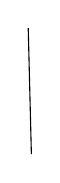
\begin{tikzpicture}[x=1cm,y=1cm]\draw (0,0)--(-0.04,1.6);\end{tikzpicture}}}
faut et il suffit qu'il existe un entier $n>0$, et un hom. de schémas en groupes $\varphi:\mathbb G_a\longrightarrow G$, tel qu'on ait
\[
(13)\qquad \varphi(1)=g^n.
\]

La suffisance étant triviale, il s'agit d'examiner la nécessité. Pour simplifier, on va encore supposer $S$ noethérien et intègre --- une fois $S$ supposé noethérien, je pense que la réduction au cas intègre doit se faire par des dévissages faciles, que je n'ai pas envie de faire, faute de besoin essentiel ! Je vais donc examiner le cas $S$ noeth. intègre, pt générique $\eta$

a) Car. \unsure{de} $\eta$ est $>0$. Alors \deleted{$\unsure{g_\eta}$} l'hypothèse sur $g_\eta$ est que $g_\eta$ est d'ordre fini --- donc $\exists n>0$ tel que $g_\eta^n=1$, donc $g^n=1$. On prendra donc dans (13) cet $n$, et $\varphi$ l'hom. trivial.

b) Cas où $\eta$ est car. nulle. Soit $\varphi$
\[
(14)\qquad \varphi_{1\eta}:\mathbb G_{a\eta}\longrightarrow G_\eta
\]
défini par la condition
\[
g_\eta=\varphi_{1\eta}(1)
\]
soit $U_1$ son ``ouvert de définition'' dans $S$.

Soit
\[
\varphi_{n\eta}(\lambda)=\lambda^n=\varphi_{1\eta}(n\lambda):\mathbb G_{a\eta}\longrightarrow G_\eta
\]
et soit $U_n$ son ouvert de définition. On a donc
\[
(15)\qquad\varphi_{n\eta}(1)=g^n\quad\text{sur }U_n
\]
\margin{10}

% Pied de page imprimé de l'archive.
\begin{center}
\small
10\\
\texttt{https://grothendieck.umontpellier.fr}\\
Université de Montpellier, UMR CNRS 5149, Case courrier 051, Place Eugène Bataillon\\
34095 Montpellier cedex 5 - France
\end{center}

\scanpage{12}
\deleted{\mspage{653}}
et
\[
(16)\qquad n\mid n'\quad\Longrightarrow\quad U_n\subset U_{n'}.
\]
Il faut prouver que la réunion des $U_n$ est $S$. On est ramené au cas $S$ local, et où $\varphi_1$ est déjà défini dans
\[
(17)\qquad U_1=S\setminus\{s\},\qquad s\text{ le pt fermé de }S
\]
et ceci revient au

\margin{\unsure{à}}
\uline{Lemme} \unsure{(!)|(?)} \unsure{Soient} $S$ noeth. intègre, $G$ schéma en groupes \inserted{séparé} loc. de prés. finie sur $S$, $U$ ouvert non vide de $S$, $\varphi_U:\mathbb G_{aU}\longrightarrow G_U$ un hom. de groupes, on suppose que $\varphi_U(1)=g_U$ se prolonge en une section $g$ de $G$ sur $S$ \unsure{tt|$\forall$} entier (\unsure{néc\textsuperscript{t}.} unipotente, d'après des résultats connus généraux \unsure{de|du} SGA 3) Alors il existe un entier $>0$ tel que $\varphi_U^n:\lambda\longmapsto\varphi_U(\lambda^n)$ se prolonge \unsure{en|sur} $S$ un hom.
\[
\varphi_n:\mathbb G_a\longrightarrow G.
\]

Je ne vais pas essayer de le démontrer dans ce contexte général des schémas en groupes généraux, et vais me limiter, à titre de test décisif (pour emporter conviction que \unsure{ça marche}) le cas où $G=\mathrm{Gl}(n)_S$, comme tantôt, et celui où $S$ de plus est régulier de dim 1.

Donc on est ramené à la situation d'une \unsure{jauge} $A$, et de $X\in M_n(K)$ ($K$ corps des fractions) satisfaisant
\margin{11}

% Pied de page imprimé de l'archive.
\begin{center}
\small
11\\
\texttt{https://grothendieck.umontpellier.fr}\\
Université de Montpellier, UMR CNRS 5149, Case courrier 051, Place Eugène Bataillon\\
34095 Montpellier cedex 5 - France
\end{center}

\scanpage{13}
\mspage{\textcircled{654}}
\[
(18)\qquad
\left\{\begin{array}{l}
X\in M_n(K)\\
X^n=0,\quad\displaystyle\sum\frac{X^i}{i!}\in M_n(A),\quad
\displaystyle\sum\frac{(-1)^iX^i}{i!}\in M_n(A)
\end{array}\right.
\]
et on veut montrer qu'il existe un entier $d>0$ tel qu'on ait
\[
(19)\qquad\frac{d^iX^i}{i!}\in M_n(A)\qquad(1\leq i\leq n-1)
\]
Si $A$ est de car 0 i.e. s'il est une $\mathbb Q$-algèbre, ceci \deleted{implique} \inserted{est équivalent} d'ailleurs :
\[
\frac{X^{\deleted{\unsure{i|0}}}}{\deleted{\unsure{i!}}}\in M_n(A)
\qquad\deleted{\text{\illegible{1}}\ X^i\in M_n(A))}
\]
\margin{\figure{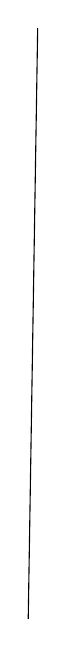
\begin{tikzpicture}[x=1cm,y=1cm]\draw (0,0)--(0.12,7.5);\end{tikzpicture}}}
\margin{le cas de car. nulle se \unsure{résout|résoud} par l'affirmative à l'aide de la fonction logarithme --- \unsure{posant|prenant}
\[
X+\frac{X^2}{2!}+\cdots+\frac{X^{n-1}}{(n-1)!}=Y,
\]
on aura
\[
\exp X=1+Y,\quad\text{donc}
\]
\[
X=\log(1+Y)=Y-\frac{Y^2}{2}+\frac{Y^3}{3}\ldots
\]
Marche sur un anneau de base quelconque de car nulle\ldots}
\margin{$\unsure{b|0}$}
i.e. Il faudrait que dans le cas de car. 0, c'est $\varphi_U$ lui-$\overline{\mathrm m}$ qui puisse déjà se prolonger à $S$ tout entier. Le premier cas douteux à ce sujet me semble $\unsure{n|m}=5$
\[
(20)\qquad\left\{\begin{array}{l}
\deleted{\unsure{X^5=0}}\quad\inserted{X\in M_5(\unsure{A|K}),\ X^5=0}\\
\displaystyle\frac{X^2}{2}\pm\frac{X^3}{\unsure{3!|6!}}+\frac{X^4}{\deleted{\unsure{2}}4!}\in M_5(A)\\[3pt]
\overset{?}{\Longrightarrow}\quad\deleted{\unsure{X^2,X^3,X^4}}\quad X\in M_5(A)
\end{array}\right.
\]

Par contre, dans le cas envisagé un peu précédemment ($n=4$, car. résiduelle 2 --- le seul qui fasse des difficultés) il est clair qu'il suffit de prendre pour $d$ une puissance de 2 assez grande.

Cette remarque s'applique aux cas d'inégales caractéristiques. On doit avoir en fait ceci

\uline{Corollaire au lemme} \unsure{dubitatif} : si $S$ est local, de car. résiduelle $p>0$, et si $\varphi$ est défini sur un ouvert qui contient $S-V(p)$, (i.e. si le complémentaire de $U$ est de car. $p\unsure{>|\geq}0$ --- en fait inutile bien sûr que $S$ soit local) alors $\exists q=p^{\unsure{r|n}}$ tel que $\varphi^q$ se prolonge.
\margin{12}

% Pied de page imprimé de l'archive.
\begin{center}
\small
12\\
\texttt{https://grothendieck.umontpellier.fr}\\
Université de Montpellier, UMR CNRS 5149, Case courrier 051, Place Eugène Bataillon\\
34095 Montpellier cedex 5 - France
\end{center}

\scanpage{14}
Quand $G$ est affine, ceci devrait être trivial. On va essayer la

\uline{Proposition} \unsure{Soient|Soit} $S$ un préschéma qu. cpt, $n$ un entier $\unsure{\geq1|\geq0}$, \deleted{\unsure{premier|prem.}} $S_0=V(n)\subset S$ le sous-schéma fermé défini par $n.1_S$ (donc si $x\in S$, on a $x\in S_0$ ssi \deleted{\unsure{car. $x$ est de}} \deleted{\unsure{car qui divise $n$}} \inserted{car $x\mid n$}), \inserted{$U=S\setminus S_0$,} $G$ un schéma en groupes affine \inserted{de \unsure{p.f.|t.f.}} sur $S$, et
\[
(21)\qquad\varphi_U:\mathbb G_a|U\longrightarrow G|U
\]
un hom. de groupes. \inserted{On suppose $U$ schématiquement dense dans $S$.} Alors il existe une \inserted{puiss.} entier \deleted{$d>0$} \inserted{$m=n^{\unsure{r|\nu}}$ de $n$,} \deleted{tel que} et un hom. de schémas en groupes
\[
\psi_m:\mathbb G_a\longrightarrow G\unsure{;|,}
\]
tel qu'on ait
\[
(22)\qquad\psi_m|U=\bigl(\varphi_U^m:\lambda\longmapsto\varphi_U(\unsure{m\lambda})=\varphi_U(\lambda)^m\bigr)
\]
Considérons en effet l'endom
\[
u_m:\mathbb G_a\longrightarrow\mathbb G_a\qquad\lambda\longmapsto m\lambda
\]
Alors la formule (22) signifie qu'on a commutativité
\diagram{\begin{tikzcd}
\mathbb G_{aU}\arrow[r,dash,"(u_m)_U"]\arrow[dr,"\psi_U"']&\mathbb G_{aU}\arrow[d,"\varphi_U"]\\
&G_U
\end{tikzcd}}
et l'existence des $\unsure{\psi_i|\psi_m}$ pour $m$ grand, signifie que pour $m$ grand l'hom. composé
\[
\deleted{\varphi_U\circ u_m}\qquad\varphi_U\circ u_m:\mathbb G_{aU}\unsure{\longrightarrow|\text{---}}G_U
\]
se prolonge en un hom. de groupes $\mathbb G_a\longrightarrow G$.
\margin{13}

% Pied de page imprimé de l'archive.
\begin{center}
\small
13\\
\texttt{https://grothendieck.umontpellier.fr}\\
Université de Montpellier, UMR CNRS 5149, Case courrier 051, Place Eugène Bataillon\\
34095 Montpellier cedex 5 - France
\end{center}

\scanpage{15}
\mspage{655}

Pour raisons de densité schématique et \unsure{unicité},
il suffit de prouver que $\varphi_U$ se prolonge en un
hom de schémas \deleted{en groupes} -- \inserted{ce} prolongement sera
automatiquement un hom de sch. en groupes.
\deleted{$A$ \unsure{celui de} \illegible{1} $B$}
\inserted{OPS $S$ \unsure{Affine}, \unsure{soit}}
$A$ \unsure{son} anneau, et soit $B$ celui de $G$.
Donc l'anneau de $U$ sera
\deleted{$A[1/n]\unsure{=}$}
$A_n\overset{\unsure{\mathrm{déf}}}{=}A[1/n]$, celui de $G$ sera
$B\otimes_A A_n=B_n$, par hyp on a un hom
(correspondant à $\unsure{\varphi_U^*|\varphi_U}$)
\[
(23)\qquad
\diagram{\begin{tikzcd}
B_n \arrow[r,"\varphi"] & A_n[T]
\end{tikzcd}}
\]
tandis que l'hom \deleted{\unsure{composé}}
\inserted{correspondant} à $\psi_{mU}$ sera le composé du précédent
avec
\[
(24)\qquad
\diagram{\begin{tikzcd}
A_n[T] \arrow[r,"\unsure{\psi_m^*|u_m^*}"] & A_n[T] \\
T \arrow[r,mapsto] & mT & \text{donc} & T^i \arrow[r,mapsto] & m^iT^i
\end{tikzcd}}
\]
Soit \deleted{$\unsure{x}$}
$\inserted{x=}\,a_0+a_1T+\cdots+a_NT^N\in A_n[T]$ \unsure{dont|donc} les
$a_i\in A_n$ on aura donc
\[
\psi_m^*(x)=\sum a_i m^iT^i=\sum(a_i n^{\unsure{i\nu}})T^i
\]
donc si $m=n^\nu$ est assez grand, on aura
\[
\deleted{\psi_m^*(x)\unsure{\sim}m^iT^i\in\unsure{A}}
\]
\[
m^i a_i\in A\quad\text{i.e}\quad m^i a_i\in\unsure{A|T^i}[T]
\qquad \forall i\,\uuline{\unsure{\ge|>}1}
\]
donc
\[
\psi_m^*(x)\equiv a_0\pmod{A[T]}
\]
ce qui montre
\[
(25)\qquad \psi_m(x)\in A[T]\ \text{pour }m=n^\nu\text{ grand}
\quad\Longleftrightarrow\quad a_0\in A
\]
\margin{14}

% Pied de page imprimé de l'archive.
\begin{center}
\small
14\\
\texttt{https://grothendieck.umontpellier.fr}\\
Université de Montpellier, UMR CNRS 5149, Case courrier 051, Place Eugène Bataillon\\
34095 Montpellier cedex 5 - France
\end{center}

\scanpage{16}

Appliquant ceci aux images d'éléments de $B$ qui engendrent $B$ comme
$A$-algèbre, on a donc

\uline{Corollaire}\quad $S$ \deleted{$\unsure{S_0}$} $n,S_0,U$ étant comme dans
la proposition, et $G$ étant un schéma affine de t.f. sur $S$
(il n'est plus question de structure de groupes), et
$\varphi_U:\mathbb E^1_U\longrightarrow G_U$ un hom de schémas,
\deleted{pour qu'il \unsure{existe}}
$g_U\,\deleted{\unsure{=}}\overset{\unsure{\mathrm{déf}}}{=}\varphi_U(0)$,
Pour qu'il existe une \deleted{\illegible{1}} puissance $m=n^\nu$
de $n$ telle que $\varphi_U\circ\unsure{\psi_m|u_m}$
\deleted{\unsure{(où}} (où $u_m$ donné par (24)) se prolonge
\inserted{à $S$}, il f et s. que $g_U$ se prolonge en une section $g$ de $G$
sur $S$.

\uline{Remarque}\quad les arguments précédents prouvent
en tous cas le "théorème" \unsure{dubitatif} p.\unsure{662|652}!
dans le cas où $S$ est noeth. de dim. 1
(le cas intéressant pour nous étant celui où le pt générique de $S$
est de car. 0).

\margin{\uline{Schémas en groupes} \uline{associés à des}
\unsure{ext. de} \uline{groupes discrets}}

3.\quad Soit maintenant $\unsure{M_0|M}$ un $\mathbb Z$-module
libre de type fini; on va construire un
pro-schéma en \uline{groupes} sur $S$, associé
au syst. projectif des sous-\deleted{groupes}\inserted{$\mathbb Z$}-modules
d'indice fini de $M$. Pour faire la
construction, je vais développer \deleted{\unsure{donc}} une
\margin{15}

% Pied de page imprimé de l'archive.
\begin{center}
\small
15\\
\texttt{https://grothendieck.umontpellier.fr}\\
Université de Montpellier, UMR CNRS 5149, Case courrier 051, Place Eugène Bataillon\\
34095 Montpellier cedex 5 - France
\end{center}

\scanpage{17}
\mspage{656}

\margin{Je me \unsure{complique} l'existence pour la construction de
$\underline{\unsure{\mathcal G}}$, il suffit de poser
$\underline{\unsure{\mathcal G}}=
\unsure{\mathcal G}_{S_0}\times_{M_{S_0}}\underline M_{S_0}$.}

\unsure{gamme|lemme} préliminaire, relatif à une situation
\[
(26)\qquad
\diagram{\begin{tikzcd}
1 \arrow[r] & M \arrow[r] & \unsure{\mathcal G} \arrow[r] & H \arrow[r] & 1
\end{tikzcd}}
\]
suite exacte de groupes discrets, avec $M$ commutatif --
le cas qui nous \unsure{intéressera} par la suite étant celui où $M$ est un
$\mathbb Z$-module libre de t.f. En tous cas $M$ est un
$\mathbb Z$-module, et à ce titre définit un Groupe sur
$\deleted{\unsure{\mathbb Z}}\inserted{\unsure{S_0}}=\operatorname{Spec}\mathbb Z$,
savoir
\[
\diagram{\begin{tikzcd}
A \arrow[r,mapsto] & M\otimes_{\mathbb Z}A
\end{tikzcd}}
\]
($A$, $\mathbb Z$-algèbre commutative) -- qu'on va désigner par $\underline M$.
En fait, $\underline M$ est représentable, i.e. est un \uline{schéma}
en groupes ssi $M$ est libre de type fini.
J'ai envie de définir aussi des \deleted{schémas en} Groupes sur $S_0$
(qui seront des schémas en groupes si $M$ l'est)
$\underline{\unsure{\mathcal G}},\underline H$, et une suite exacte
\[
(27)\qquad
\diagram{\begin{tikzcd}
1 \arrow[r] & \underline M \arrow[r] &
\underline{\unsure{\mathcal G}} \arrow[r] & \underline H \arrow[r] & 1
\end{tikzcd}}
\]
de Groupes sur $S_0$, et un isom des suites exactes
\[
(28)\qquad
\diagram{\begin{tikzcd}
1 \arrow[r] & M \arrow[r] \arrow[d,"\unsure{\wr}"] &
\unsure{\mathcal G} \arrow[r] \arrow[d,"\unsure{\wr}"] &
H \arrow[r] \arrow[d,"\unsure{\wr}"] & 1 \\
1 \arrow[r] & \underline M(\mathbb Z) \arrow[r] &
\underline{\unsure{\mathcal G}}(\mathbb Z) \arrow[r] &
\underline H(\mathbb Z) \arrow[r] & 1
\end{tikzcd}}
\]
on prendra
\[
(29)\qquad \underline H=H_{S_0}
\qquad\text{Groupe constant de val. }H
\]
et les flèches verticales extrêmes de (28)
\margin{16}

% Pied de page imprimé de l'archive.
\begin{center}
\small
16\\
\texttt{https://grothendieck.umontpellier.fr}\\
Université de Montpellier, UMR CNRS 5149, Case courrier 051, Place Eugène Bataillon\\
34095 Montpellier cedex 5 - France
\end{center}

\scanpage{18}

\unsure{seront|sont} les isom. canoniques.

On peut songer à définir $\underline{\unsure{\mathcal G}}$ comme
foncteur \inserted{(cov.)} en $A/\mathbb Z$ ou (\unsure{contravariant})
en $S/S_0$, par
\[
(30)\qquad
\underline{\unsure{\mathcal G}}(A)=
\unsure{\mathcal G}\wedge_M
\underbrace{M(A)}_{\deleted{\unsure{A\otimes_{\mathbb Z}}}\inserted{M\otimes_{\mathbb Z}A}}
\]
\deleted{\unsure{Comme on a}}.
$\underline{\unsure{\mathcal G}}(A)$ étant donc défini comme l'ext. de
$H$ par $M(A)$ \unsure{déduite} de l'ext. $\unsure{\mathcal G}$
de $H$ par $M$ par l'hom
\[
(31)\qquad
\diagram{\begin{tikzcd}
M \arrow[r] & M\otimes_{\mathbb Z}A
\end{tikzcd}},
\]
qu'on considère comme un hom de $H$-$\mathbb Z$-modules,
en faisant opérer $H$ sur $M\otimes_{\mathbb Z}A$ via son opération sur $M$.

La petite difficulté est que le foncteur-\unsure{groupe|groupes}
ainsi défini par (30) n'est pas lui-$\overline{\mathrm m}$ représentable --
il ne donne l'expression correcte de $\underline{\unsure{\mathcal G}}(A)$ que si
$\operatorname{Spec}A$ est connexe -- il correspond au sous-foncteur de
\[
\begin{array}{c}
\inserted{\unsure{\sim}}\\[2pt]
\diagram{\begin{tikzcd}
S \arrow[r,mapsto] &
\unsure{:}\underline{\unsure{\mathcal G}}(A)=
\deleted{\unsure{\operatorname{Spec}|\underline{\mathcal G}}}
\underline{\unsure{\mathcal G}}(S)
\end{tikzcd}}
\qquad (S=\operatorname{Spec}A)
\end{array}
\]
formé des \deleted{pts tels que le}
\inserted{$S\longrightarrow\underline{\unsure{\mathcal G}}$}
tels que le composé
\[
(32)\qquad
\diagram{\begin{tikzcd}
S \arrow[r] & \underline H_S
\end{tikzcd}}
\]
(qui correspond à une fonction \uuline{loc.} \uline{\unsure{constante|const.}}
sur $S$ à valeurs dans $H$) soit
\inserted{(\unsure{entièrement})} constante.
\margin{17}

% Pied de page imprimé de l'archive.
\begin{center}
\small
17\\
\texttt{https://grothendieck.umontpellier.fr}\\
Université de Montpellier, UMR CNRS 5149, Case courrier 051, Place Eugène Bataillon\\
34095 Montpellier cedex 5 - France
\end{center}

\scanpage{19}
\mspage{657}

L'expression correcte s'obtiendra en partant du \unsure{"}foncteur incorrect"
\[
\diagram{\begin{tikzcd}
{[\underline{\unsure{\mathcal G}}]: A} \arrow[r,mapsto] &
\unsure{\mathcal G}\wedge_M(M\otimes_{\mathbb Z}A)
\end{tikzcd}}
\]
\unsure{ou} mieux, du \unsure{contr. foncteur|contre-foncteur}
\[
\diagram{\begin{tikzcd}
S \arrow[r,mapsto] &
\unsure{\mathcal G}\wedge_M
\Gamma(S,M\otimes_{\mathbb Z}\underline{\unsure{\mathcal O|O}}_S)
\end{tikzcd}},
\]
et en prenant le faisceau Zariski associé -- en fait on aura. $=$
\[
(33)\qquad
\underline{\unsure{\mathcal G}}(S)=
\underset{\mathcal U=(U_i)_{i\in\unsure{S|I}}}{\varinjlim}
\prod_{i\in I}[\unsure{\mathcal G}](U_i)
\]
\[
\begin{array}{l}
(U_i)_{i\in I}\ \text{une partition}\\
\text{de }S\text{ en }\unsure{\text{schém.}}\\
\unsure{\text{ouverts}}\qquad S\simeq\coprod U_i
\end{array}
\]

Voici une autre façon de présenter la construction de
$\underline{\unsure{\mathcal G}}$, en utilisant la construction générale
du §49 -- dans le contexte faisceautique. On a un système
\[
(34)\qquad
\underbrace{\underline M}_{\text{Groupe sur }S_0},
\quad
\underbrace{\unsure{\mathcal G}_{S_0}
\overset{\cdot}{\supset}\unsure{M}_{S_0}}_{
\substack{\text{Groupes (constants)}\\
\text{sur }S_0,\ M_{S_0}\\
\text{distingué}}},
\quad
\mathrm{Op.}^{\unsure{\Theta|\theta}}\text{ de }
\unsure{\mathcal G}_{S_0}\text{ sur }\underline M,
\]
\[
\diagram{\begin{tikzcd}
\text{hom }\varphi:
\deleted{\unsure{\mathcal G}}\inserted{M}_{S_0}
\arrow[r] & \underline M
\end{tikzcd}}
\]
(où l'op. de $\unsure{\mathcal G}_{S_0}$ sur $\underline M$,
qui \unsure{revient} à une op. de $\unsure{\mathcal G}$ sur $\underline M$,
est celle déduite de l'op. de $\unsure{\mathcal G}$ sur $M$,
par \unsure{fonctorialité})
ces données \unsure{satisfaisant} aux conditions de compatibilité a) b)
de loc. cit. Par la construction \unsure{du|de} loc. cit., on construit
\margin{18}

% Pied de page imprimé de l'archive.
\begin{center}
\small
18\\
\texttt{https://grothendieck.umontpellier.fr}\\
Université de Montpellier, UMR CNRS 5149, Case courrier 051, Place Eugène Bataillon\\
34095 Montpellier cedex 5 - France
\end{center}
